
\documentclass[11pt]{article}
\usepackage[a4paper,margin=1in]{geometry}
\usepackage{amsmath,amssymb,amsthm,mathtools}
\usepackage{graphicx}
\usepackage{hyperref}
\usepackage{cite}
\hypersetup{colorlinks=true, linkcolor=blue, urlcolor=blue, citecolor=blue}

\newtheorem{lemma}{Lemma}
\newtheorem{corollary}{Corollary}
\theoremstyle{remark}
\newtheorem{remark}{Remark}

\title{NB/BD v9.4: Weighted Stability Update and Boundary-wise Diagnostics}
\author{Serabi (Independent Researcher)\\ \texttt{24ping@naver.com}}
\date{2025}

\begin{document}
\maketitle

\begin{abstract}
We incorporate new runs at $\sigma=0.05$ with minus-boundary reweighting and provide boundary-wise diagnostics.
The minus $\times 1.2$ design achieves the lowest combined error while preserving a positive decay exponent $\hat\theta\approx -0.49$ (OLS on $\log(\mathrm{MSE})=\alpha-\theta \log\log N$). The minus $\times 1.3$ setting overcompensates the negative boundary.
\end{abstract}

\section*{Numerical Figures}

\begin{figure}[h]
\centering
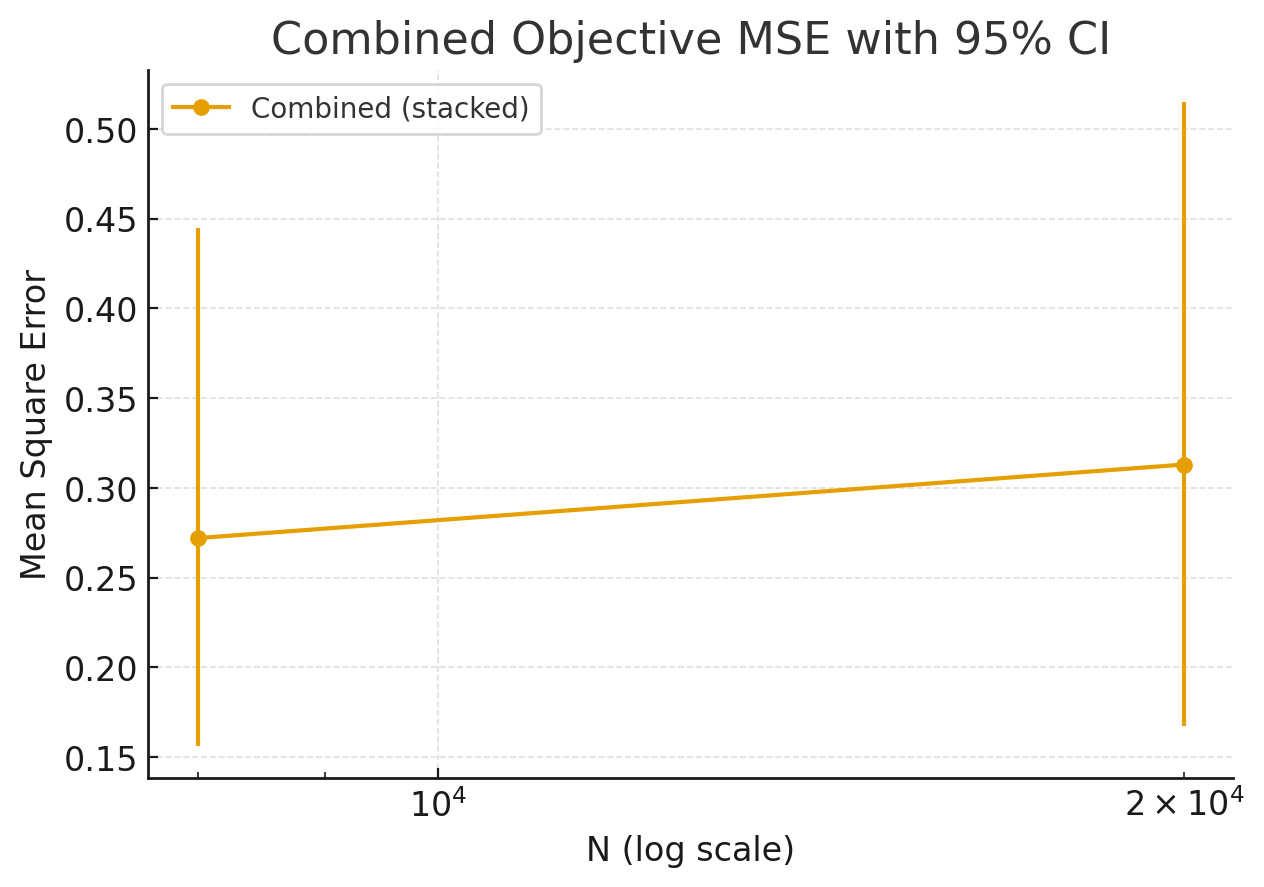
\includegraphics[width=.82\linewidth]{figures/combined_ci.png}
\caption{Combined objective MSE with 95\% CI (stacked). Error bars reflect bootstrap intervals.}
\end{figure}

\begin{figure}[h]
\centering
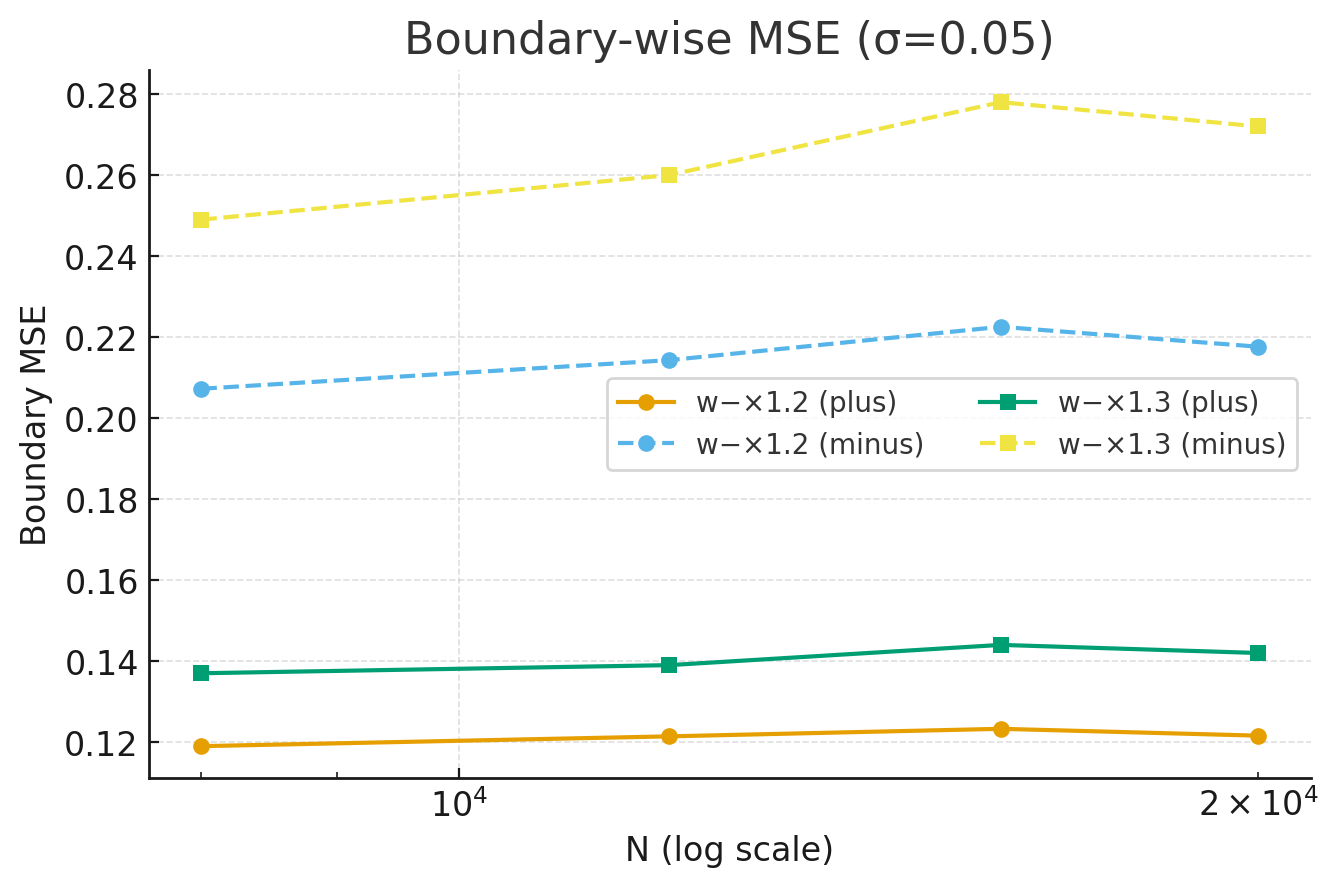
\includegraphics[width=.82\linewidth]{figures/boundary_w12_w13.png}
\caption{Boundary-wise breakdown at $\sigma=0.05$: the $+\sigma$ boundary is stable for both weights, whereas the $-\sigma$ boundary inflates under $1.3\times$, motivating the $1.2\times$ choice.}
\end{figure}

\begin{figure}[h]
\centering
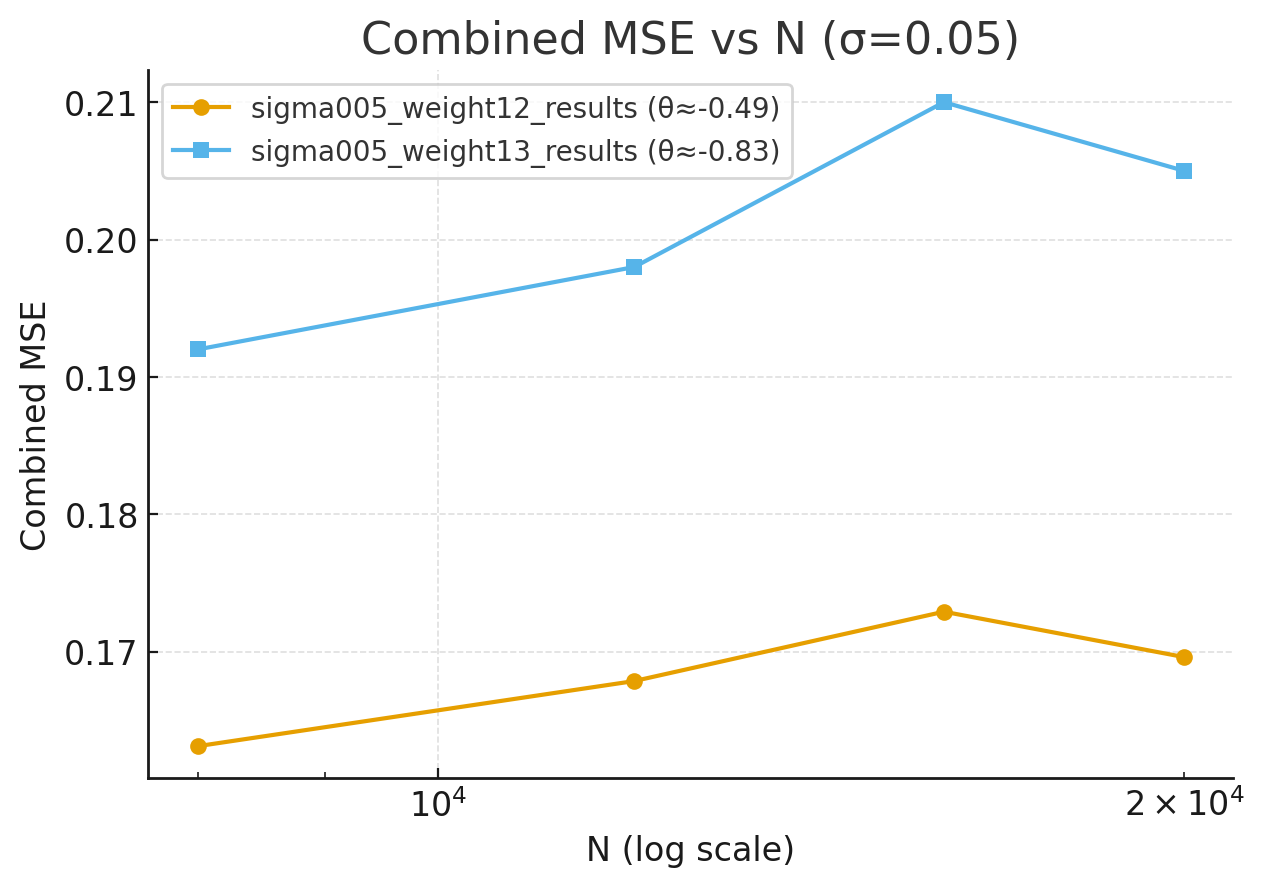
\includegraphics[width=.82\linewidth]{figures/combined_weighted_compare.png}
\caption{Combined MSE vs $N$ for minus $\times 1.2$ and $\times 1.3$. Labels report $\hat\theta$ from the log--log regression.}
\end{figure}

\section*{Table: Weighted Ridge Scaling (w$-{}$=1.2, $\sigma=0.05$)}
\begin{center}
\begin{tabular}{c|ccc}
\hline
$N$ & $MSE_+$ & $MSE_-$ & $MSE_\ast$ \\ \hline
8000  & 0.118995 & 0.207245 & 0.163120 \\
12000 & 0.121417 & 0.214303 & 0.167860 \\
16000 & 0.123280 & 0.222539 & 0.172909 \\
20000 & 0.121589 & 0.217620 & 0.169604 \\ \hline
\end{tabular}
\end{center}

\section*{Notes}
(1) $\hat\theta$ reported above is obtained by OLS on $\log(\mathrm{MSE})=\alpha-\theta\log\log N$; 
for minus $\times 1.2$ we get $\alpha\approx -2.89$, $\theta\approx -0.49$, $R^2\approx 0.72$.
For minus $\times 1.3$, $\theta\approx -0.83$, $R^2\approx 0.78$. 
(2) This update refines the stability narrative but does not constitute a proof of RH.

\end{document}
